\usetikzlibrary{positioning}
\usetikzlibrary{calc}

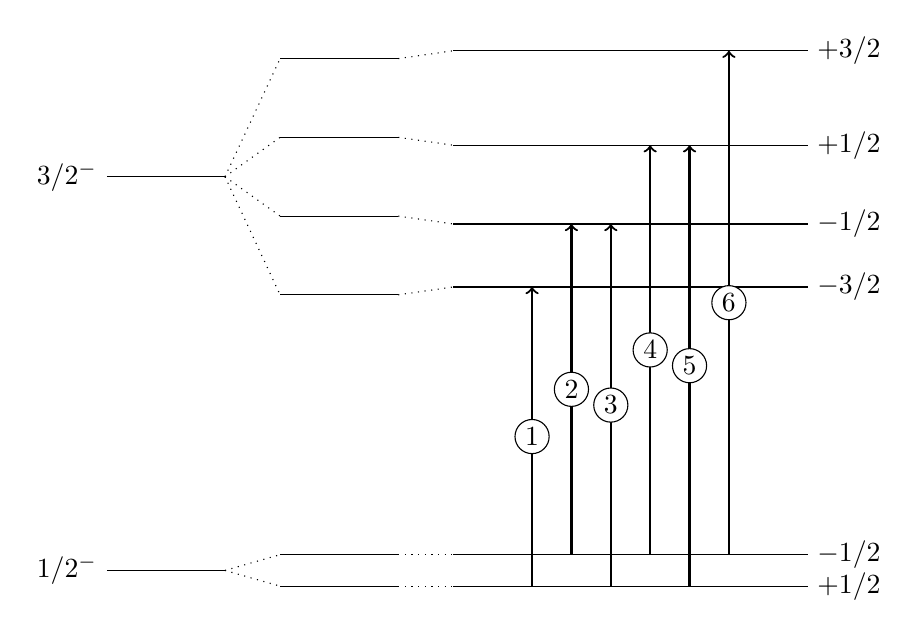
\begin{tikzpicture}[
        transition/.style={
            ->,
            thick,
        },
        number/.style={
            draw,
            thin,
            midway,
            circle,
            fill=white,
            inner sep=1.5pt,
        },
    ]
    \coordinate (a1) at (0, 0);
    \coordinate (b1) at (0, -5);

    \coordinate[right=1.5 of a1] (a1e);
    \coordinate[right=1.5 of b1] (b1e);

    \draw (a1) node[left] {$3/2^-$} to (a1e);
    \draw (b1) node[left] {$1/2^-$} to (b1e);

    % Define levels with magnetic splitting.
    \coordinate[above right=1.5 and 0.7 of a1e] (c1);

    \coordinate[below=1 of c1] (c2);
    \coordinate[below=1 of c2] (c3);
    \coordinate[below=1 of c3] (c4);

    \coordinate[right=1.5 of c1] (c1e);
    \coordinate[right=1.5 of c2] (c2e);
    \coordinate[right=1.5 of c3] (c3e);
    \coordinate[right=1.5 of c4] (c4e);

    \coordinate[above right=0.2 and 0.7 of b1e] (d1);

    \coordinate[below=0.4 of d1] (d2);

    \coordinate[right=1.5 of d1] (d1e);
    \coordinate[right=1.5 of d2] (d2e);

    % Draw levels.
    \draw (c1) to (c1e);
    \draw (c2) to (c2e);
    \draw (c3) to (c3e);
    \draw (c4) to (c4e);

    \draw (d1) to (d1e);
    \draw (d2) to (d2e);

    % Draw splitting.
    \draw[dotted] (a1e) to (c1);
    \draw[dotted] (a1e) to (c2);
    \draw[dotted] (a1e) to (c3);
    \draw[dotted] (a1e) to (c4);

    \draw[dotted] (b1e) to (d1);
    \draw[dotted] (b1e) to (d2);

    % Define levels with quadropole shift.
    \coordinate[above right=0.1 and 0.7 of c1e] (e1);
    \coordinate[below right=0.1 and 0.7 of c2e] (e2);
    \coordinate[below right=0.1 and 0.7 of c3e] (e3);
    \coordinate[above right=0.1 and 0.7 of c4e] (e4);

    \coordinate[below right=0 and 0.7 of d1e] (f1);
    \coordinate[below right=0 and 0.7 of d2e] (f2);

    \coordinate[right=4.5 of e1] (e1e);
    \coordinate[right=4.5 of e2] (e2e);
    \coordinate[right=4.5 of e3] (e3e);
    \coordinate[right=4.5 of e4] (e4e);

    \coordinate[right=4.5 of f1] (f1e);
    \coordinate[right=4.5 of f2] (f2e);

    % Draw levels.
    \draw (e1) to (e1e) node[right] {$+3/2$};
    \draw (e2) to (e2e) node[right] {$+1/2$};
    \draw (e3) to (e3e) node[right] {$-1/2$};
    \draw (e4) to (e4e) node[right] {$-3/2$};
                                            
    \draw (f1) to (f1e) node[right] {$-1/2$};
    \draw (f2) to (f2e) node[right] {$+1/2$};

    % Draw splitting.
    \draw[dotted] (c1e) to (e1);
    \draw[dotted] (c2e) to (e2);
    \draw[dotted] (c3e) to (e3);
    \draw[dotted] (c4e) to (e4);

    \draw[dotted] (d1e) to (f1);
    \draw[dotted] (d2e) to (f2);


    \draw[transition] ($(f2)+(1.0,0)$)-- node[number] {1} ($(e4)+(1.0,0)$);
    \draw[transition] ($(f1)+(1.5,0)$)-- node[number] {2} ($(e3)+(1.5,0)$);
    \draw[transition] ($(f2)+(2.0,0)$)-- node[number] {3} ($(e3)+(2.0,0)$);
                                                                     
    \draw[transition] ($(f1)+(2.5,0)$)-- node[number] {4} ($(e2)+(2.5,0)$);
    \draw[transition] ($(f2)+(3.0,0)$)-- node[number] {5} ($(e2)+(3.0,0)$);
    \draw[transition] ($(f1)+(3.5,0)$)-- node[number] {6} ($(e1)+(3.5,0)$);


\end{tikzpicture}
